\documentclass[aspectratio=169]{beamer}
\usetheme{Madrid}
\usecolortheme{default}
\usepackage{booktabs}
\usepackage{graphicx}
\usepackage{amsmath}

% Auto-generated by code.ipynb -- DO NOT EDIT MANUALLY
\newcommand{\nFeatures}{5}
\newcommand{\noMaintPct}{80.3}
\newcommand{\maintPct}{19.7}
\newcommand{\tempCorr}{0.283}
\newcommand{\vibCorr}{0.113}
\newcommand{\naiveAcc}{0.80}
\newcommand{\lrAcc}{0.6352}
\newcommand{\lrPrec}{0.2974}
\newcommand{\lrRec}{0.6255}
\newcommand{\lrFone}{0.4032}
\newcommand{\lrAuc}{0.6929}
\newcommand{\lrCvMean}{0.4091}
\newcommand{\lrCvStd}{0.0060}
\newcommand{\lrFN}{1475}
\newcommand{\lrTotalPos}{3,939}
\newcommand{\lrMissPct}{37}
\newcommand{\rfAcc}{0.8913}
\newcommand{\rfPrec}{0.9989}
\newcommand{\rfRec}{0.4488}
\newcommand{\rfFone}{0.6194}
\newcommand{\rfAuc}{0.7230}
\newcommand{\rfBestEst}{100}
\newcommand{\rfBestDepth}{None}
\newcommand{\rfBestSplit}{2}
\newcommand{\rfImpA}{0.365}
\newcommand{\rfImpNameA}{temperature}
\newcommand{\rfImpB}{0.224}
\newcommand{\rfImpNameB}{vibration}
\newcommand{\rfImpC}{0.148}
\newcommand{\rfImpNameC}{humidity}
\newcommand{\rfImpD}{0.133}
\newcommand{\rfImpNameD}{energy_consumption}
\newcommand{\rfImpE}{0.131}
\newcommand{\rfImpNameE}{pressure}
\newcommand{\rfTopThreePct}{74}
\newcommand{\annAcc}{0.8831}
\newcommand{\annPrec}{0.9029}
\newcommand{\annRec}{0.4557}
\newcommand{\annFone}{0.6057}
\newcommand{\annAuc}{0.7250}
\newcommand{\annFN}{2144}
\newcommand{\annFP}{193}
\newcommand{\annValAcc}{0.8808}
\newcommand{\annValLoss}{0.4705}
\newcommand{\annBestEpoch}{90}
\newcommand{\pcaNcomp}{5}
\newcommand{\pcaVarOne}{20.2}
\newcommand{\pcaVarTwo}{20.1}
\newcommand{\pcaAcc}{0.6352}
\newcommand{\pcaPrec}{0.2974}
\newcommand{\pcaRec}{0.6255}
\newcommand{\pcaFone}{0.4032}
\newcommand{\pcaAuc}{0.6929}
\newcommand{\pcaDeltaF}{0.0000}
\newcommand{\isoAcc}{0.7476}
\newcommand{\isoPrec}{0.3644}
\newcommand{\isoRec}{0.3783}
\newcommand{\isoFone}{0.3712}
\newcommand{\isoAuc}{0.6571}
\newcommand{\isoFP}{2599}
\newcommand{\isoFN}{2449}
  % Auto-generated by code.ipynb

\definecolor{ubcblue}{RGB}{0,40,89}
\setbeamercolor{structure}{fg=ubcblue}
\setbeamercolor{title}{fg=white,bg=ubcblue}
\setbeamercolor{frametitle}{fg=white,bg=ubcblue}

\setbeamertemplate{navigation symbols}{}
\setbeamertemplate{footline}{%
  \hfill\insertframenumber/\inserttotalframenumber\hspace{4pt}\vspace{2pt}%
}

\title{Smart Manufacturing IoT-Based\\Predictive Maintenance \& Anomaly Detection}
\author{Aomsin Nimsombun \quad Colin Xiong \quad Kaoklong Panitpongpun \quad Daniel Benjamin}
\institute{Group 22 --- MANU 465, University of British Columbia}
\date{April 2026}

\begin{document}

% ============================================================
\begin{frame}
\titlepage
\end{frame}

% ============================================================
\begin{frame}{Outline}
\tableofcontents
\end{frame}

% ============================================================
\section{Problem \& Motivation}
% ============================================================

\begin{frame}{Problem \& Motivation}
\begin{itemize}
    \item \textbf{Context:} IoT sensors continuously monitor factory equipment (temperature, vibration, pressure, humidity)
    \item \textbf{Problem:} Most facilities still use reactive or scheduled maintenance
    \begin{itemize}
        \item Unplanned downtime costs hundreds of thousands of dollars per hour
        \item Unnecessary servicing wastes resources
    \end{itemize}
    \item \textbf{Goal:} Predict maintenance needs from sensor data before failures occur
    \item \textbf{Secondary goal:} Detect anomalies without labeled data (unsupervised)
\end{itemize}
\end{frame}

% ============================================================
\section{Dataset}
% ============================================================

\begin{frame}{Dataset Overview}
\textit{Smart Manufacturing IoT-Cloud Monitoring Dataset} (Kaggle)

\vspace{0.2cm}
\begin{columns}[T]
\begin{column}{0.48\textwidth}
\begin{itemize}
    \item 100,000 records, 50 machines
    \item 1-minute intervals over 69 days
    \item 13 columns total; 5 raw sensor features used
    \item Derived features excluded (data leakage)
    \item No missing values
\end{itemize}

\vspace{0.1cm}
\textbf{Key correlations with target:}
\begin{itemize}
    \item Temperature: $r = \tempCorr$
    \item Vibration: $r = \vibCorr$
\end{itemize}
\end{column}
\begin{column}{0.48\textwidth}
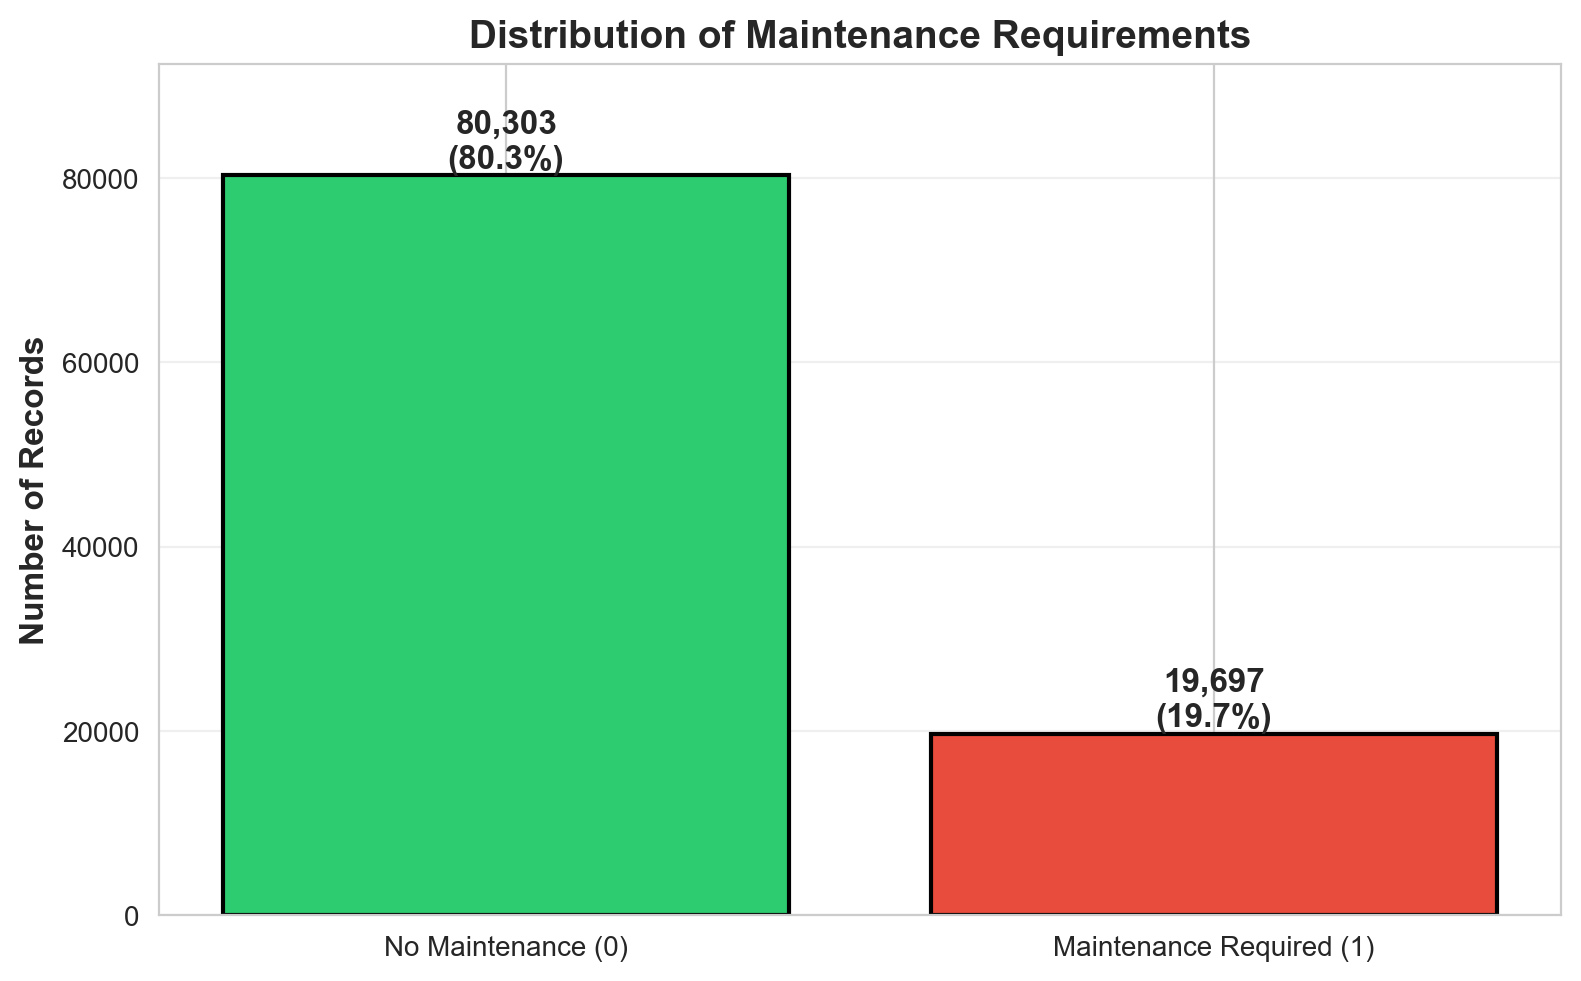
\includegraphics[width=\textwidth]{figures/class_distribution.png}
\end{column}
\end{columns}
\end{frame}

\begin{frame}{Correlation Heatmap}
\begin{center}
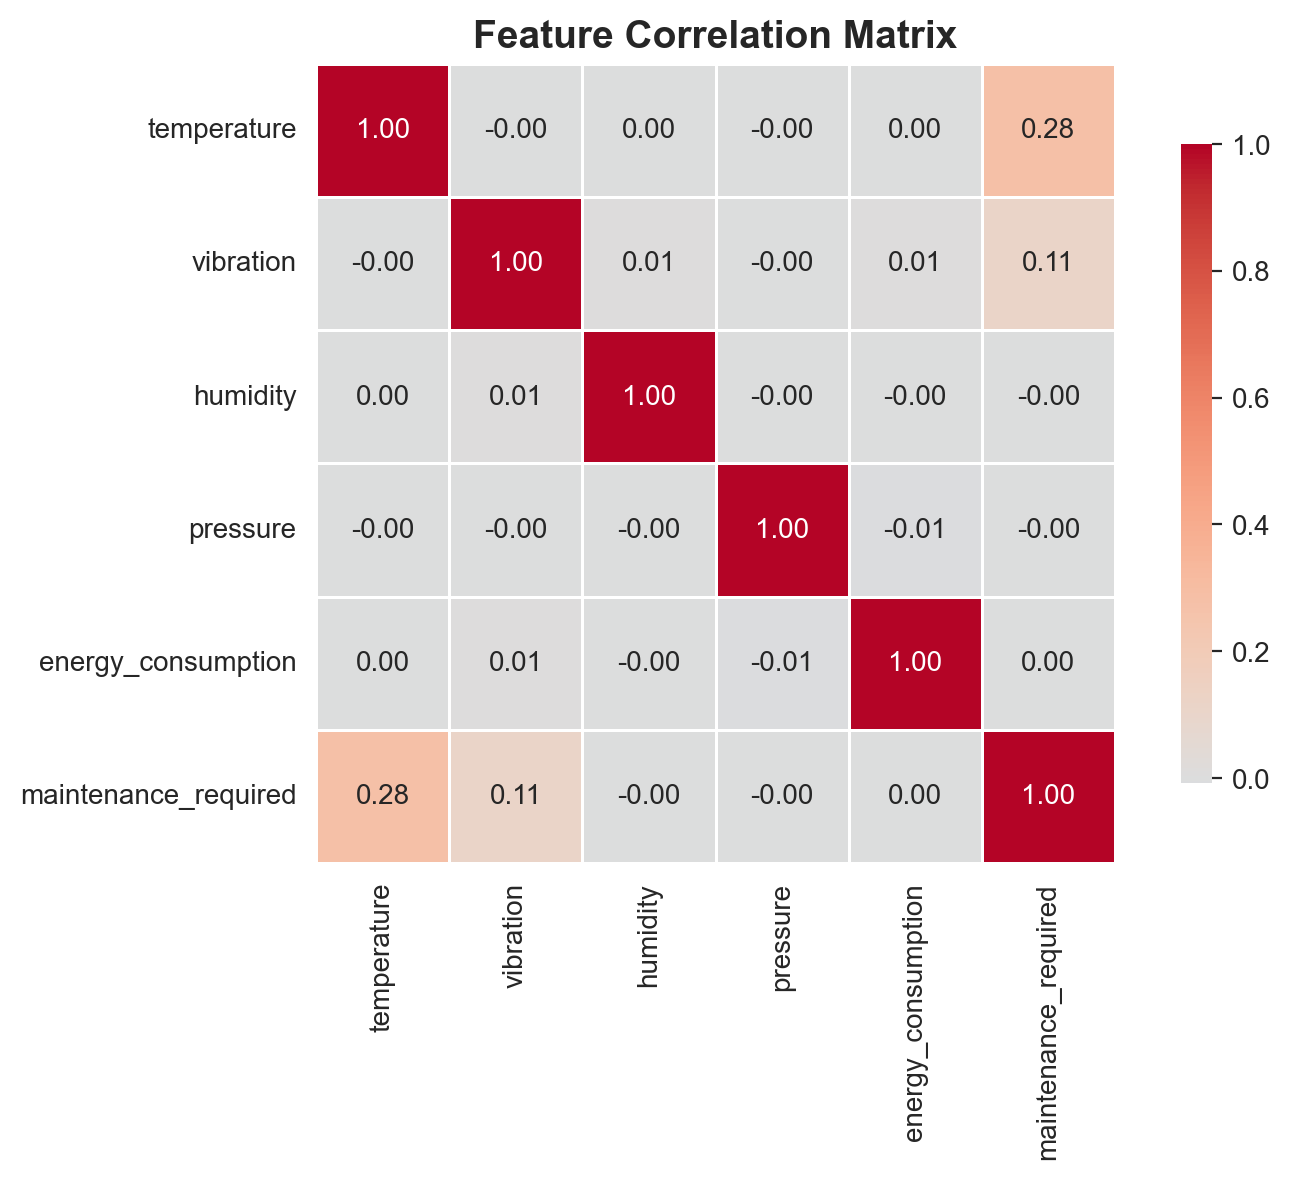
\includegraphics[width=0.48\textwidth]{figures/correlation_heatmap.png}
\end{center}
\vspace{-0.3cm}
Weak individual correlations suggest \textbf{non-linear feature combinations} are important.
\end{frame}

% ============================================================
\section{Methodology}
% ============================================================

\begin{frame}{Preprocessing}
\begin{enumerate}
    \item Dropped identifiers (\texttt{timestamp}, \texttt{machine\_id})
    \item Excluded derived features that encode the target (\texttt{machine\_status}, \texttt{anomaly\_flag}, \texttt{predicted\_remaining\_life}, \texttt{downtime\_risk}, \texttt{failure\_type})
    \item Retained 5 raw sensor features
    \item Stratified 80/20 train-test split (80k / 20k samples)
    \item StandardScaler fitted \textbf{only on training data} (prevents leakage)
    \item \texttt{class\_weight='balanced'} for imbalanced classes
\end{enumerate}
\end{frame}

\begin{frame}{ML Techniques Applied}
\begin{columns}[T]
\begin{column}{0.48\textwidth}
\textbf{Supervised:}
\begin{enumerate}
    \item \textbf{Logistic Regression} --- interpretable baseline with cross-validation
    \item \textbf{Random Forest} --- non-linear ensemble with GridSearchCV tuning
    \item \textbf{ANN (TensorFlow/Keras)} --- deep non-linear modeling with Early Stopping
\end{enumerate}
\end{column}
\begin{column}{0.48\textwidth}
\textbf{Unsupervised / Reduction:}
\begin{enumerate}
    \setcounter{enumi}{3}
    \item \textbf{PCA} --- dimensionality reduction, variance analysis
    \item \textbf{Isolation Forest} --- anomaly detection without labels
\end{enumerate}

\vspace{0.3cm}
\textbf{Evaluation metrics:}\\
Accuracy, Precision, Recall, F1, ROC-AUC, Confusion Matrices
\end{column}
\end{columns}
\end{frame}

\begin{frame}{ANN Architecture}
\begin{center}
Input (5) $\rightarrow$ Dense(64, ReLU) $\rightarrow$ Dense(32, ReLU) $\rightarrow$ Dense(16, ReLU) $\rightarrow$ Dense(1, sigmoid)
\end{center}

\vspace{0.3cm}
\begin{itemize}
    \item 3 hidden layers, Adam optimizer (lr = 0.001), binary crossentropy
    \item Early Stopping (patience = 10) with best-weight restoration
    \item Balanced class weights, batch size 256, 20\% validation split
\end{itemize}
\end{frame}

% ============================================================
\section{Results}
% ============================================================

\begin{frame}{Model Comparison}
\begin{columns}[T]
\begin{column}{0.50\textwidth}
\begin{table}
\centering
\tiny
\begin{tabular}{lccccc}
\toprule
\textbf{Model} & \textbf{Acc.} & \textbf{Prec.} & \textbf{Rec.} & \textbf{F1} & \textbf{AUC} \\
\midrule
Naive Baseline         & $\sim$\naiveAcc & --- & --- & --- & --- \\
Logistic Reg.          & \lrAcc & \lrPrec & \lrRec & \lrFone & \lrAuc \\
Random Forest          & \rfAcc & \rfPrec & \rfRec & \rfFone & \rfAuc \\
Neural Network         & \annAcc & \annPrec & \annRec & \annFone & \annAuc \\
LR + PCA               & \pcaAcc & \pcaPrec & \pcaRec & \pcaFone & \pcaAuc \\
Isolation Forest       & \isoAcc & \isoPrec & \isoRec & \isoFone & \isoAuc \\
\bottomrule
\end{tabular}
\end{table}
\end{column}
\begin{column}{0.44\textwidth}
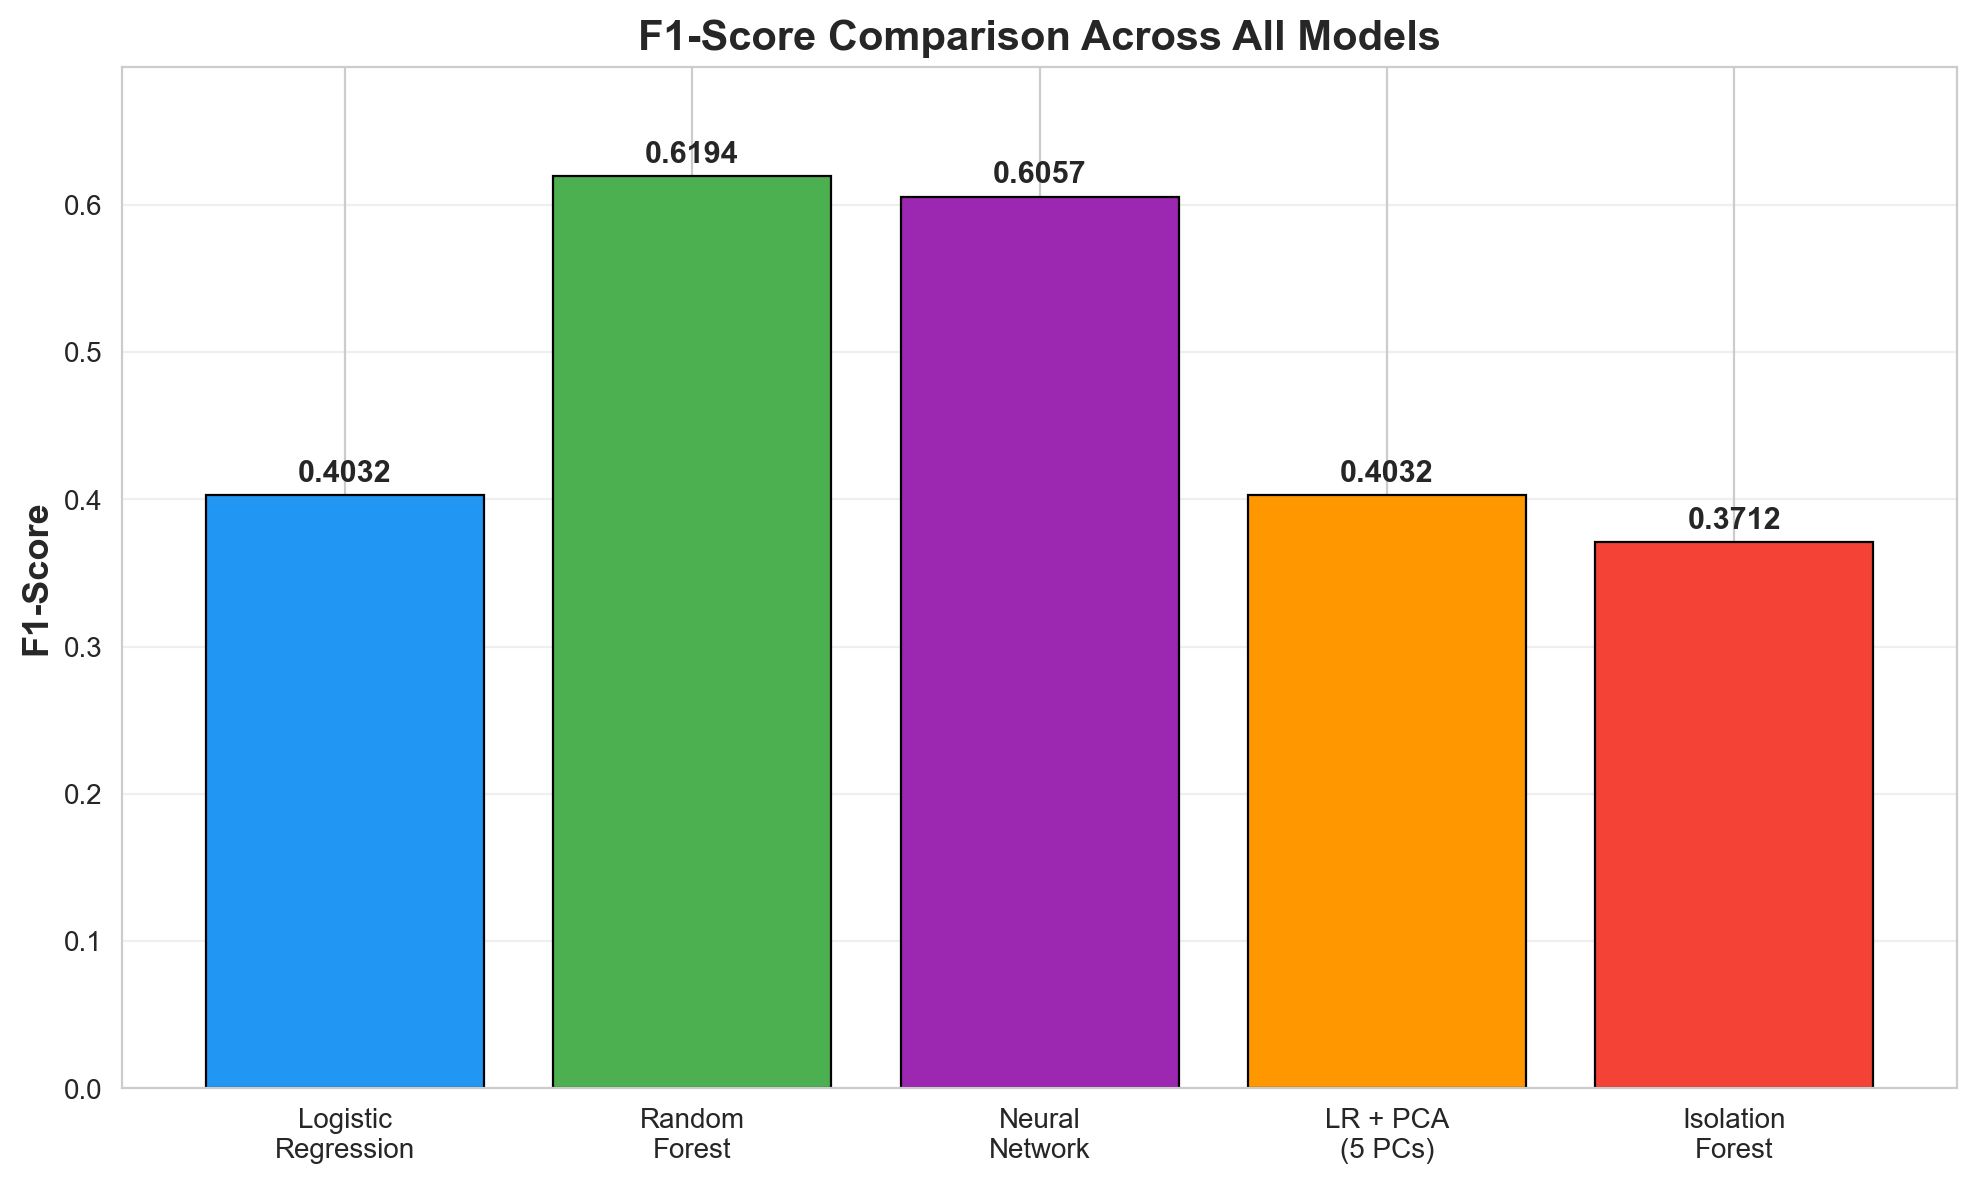
\includegraphics[width=\textwidth]{figures/f1_comparison.png}
\end{column}
\end{columns}

\vspace{0.1cm}
\begin{itemize}\small
    \item Non-linear models (RF, ANN) achieve F1 $\approx$ 0.62 vs.\ LR's \lrFone
    \item RF and ANN reach nearly identical AUC --- performance ceiling with 5 raw sensors
\end{itemize}
\end{frame}

\begin{frame}{Key Results: Logistic Regression \& Random Forest}
\begin{columns}[T]
\begin{column}{0.48\textwidth}
\textbf{Logistic Regression:}\\[2pt]
{\small
\begin{itemize}\setlength{\itemsep}{1pt}
    \item Accuracy \lrAcc\ $<$ naive \naiveAcc
    \item Recall \lrRec; precision \lrPrec
    \item CV F1: $\lrCvMean \pm \lrCvStd$
    \item Linear boundary limits performance
\end{itemize}}
\end{column}
\begin{column}{0.48\textwidth}
\textbf{Random Forest (tuned):}\\[2pt]
{\small
\begin{itemize}\setlength{\itemsep}{1pt}
    \item F1: \lrFone\ (LR) $\to$ \rfFone
    \item Precision \rfPrec\ $\approx$ perfect
    \item Recall \rfRec; misses $>$50\% of failures
    \item \rfImpNameA\ + \rfImpNameB\ = 58\% importance
\end{itemize}}
\end{column}
\end{columns}

\vspace{0.1cm}
\begin{center}
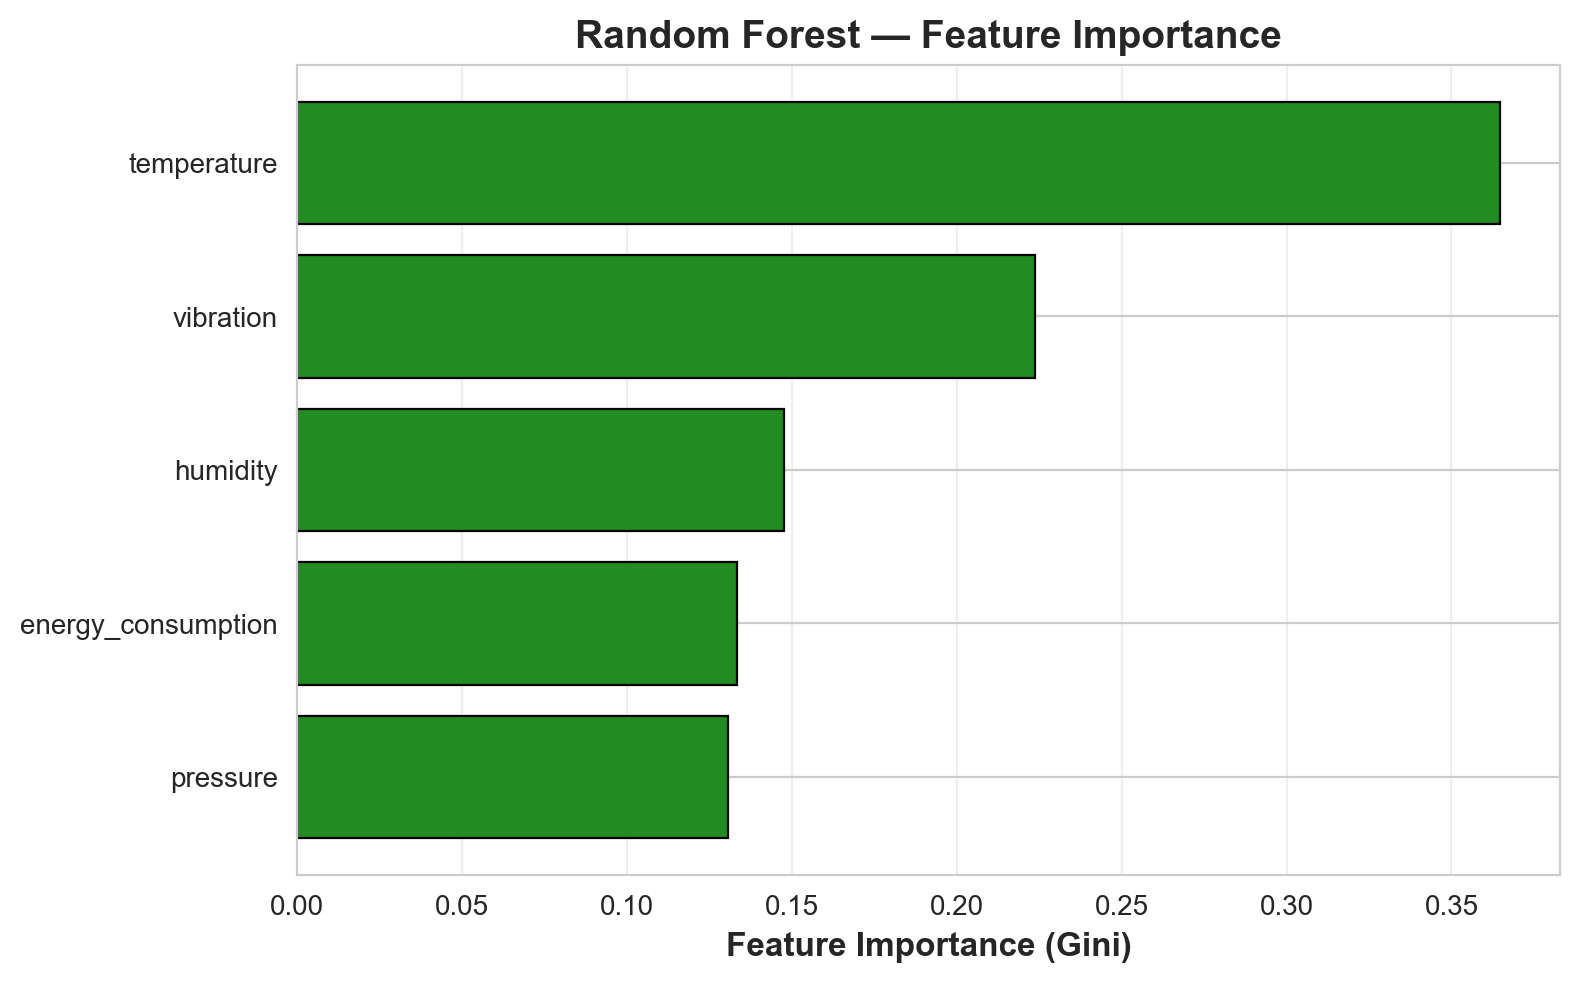
\includegraphics[width=0.40\textwidth]{figures/feature_importance.png}
\end{center}
\end{frame}

\begin{frame}{Key Results: Neural Network}
\begin{columns}[T]
\begin{column}{0.48\textwidth}
{\small
\begin{itemize}\setlength{\itemsep}{2pt}
    \item F1 = \annFone\ $\approx$ RF's \rfFone
    \item Precision \annPrec, recall \annRec
    \item \annFN\ missed failures, \annFP\ false alarms
    \item Early Stopping at epoch $\sim$\annBestEpoch
    \item AUC = \annAuc, tied with RF
\end{itemize}}
\end{column}
\begin{column}{0.48\textwidth}
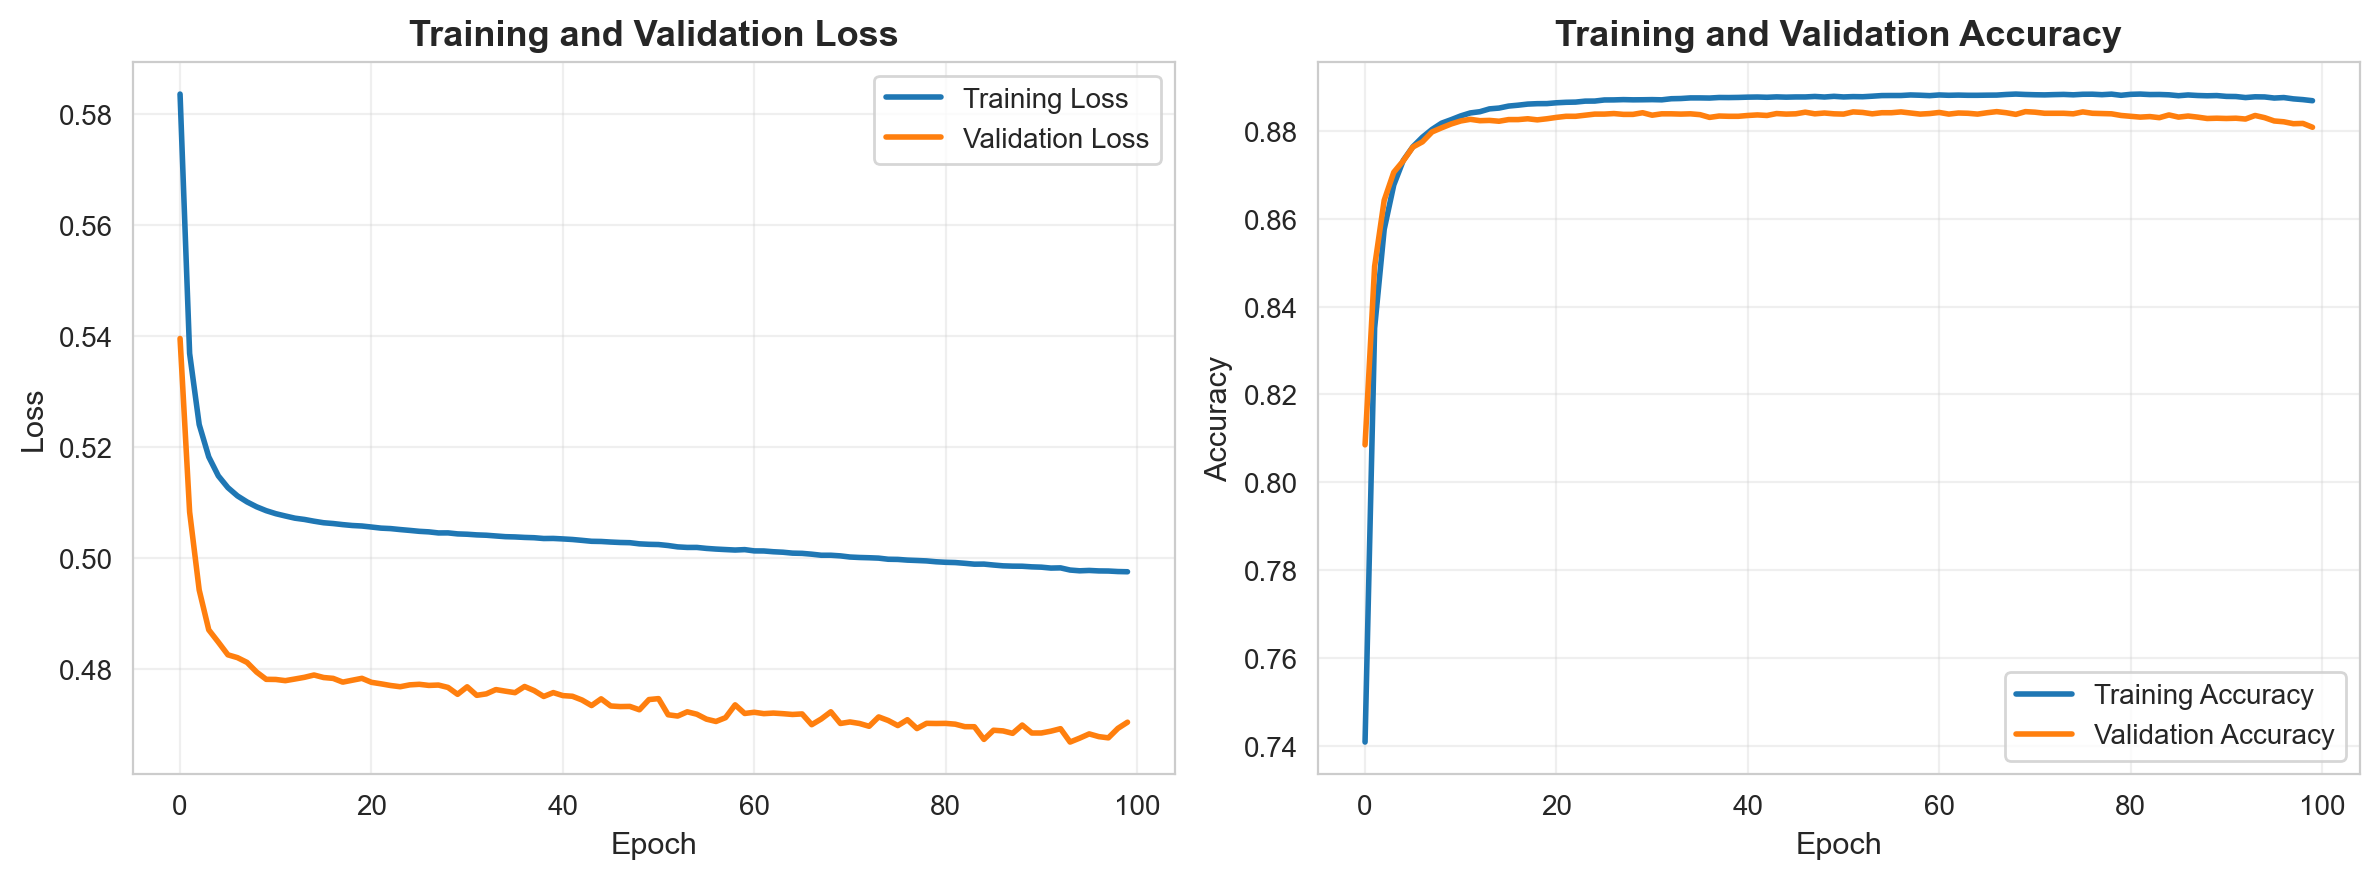
\includegraphics[width=\textwidth]{figures/ann_learning_curves.png}
\end{column}
\end{columns}
\end{frame}

\begin{frame}{Confusion Matrices — All Models}
\begin{center}
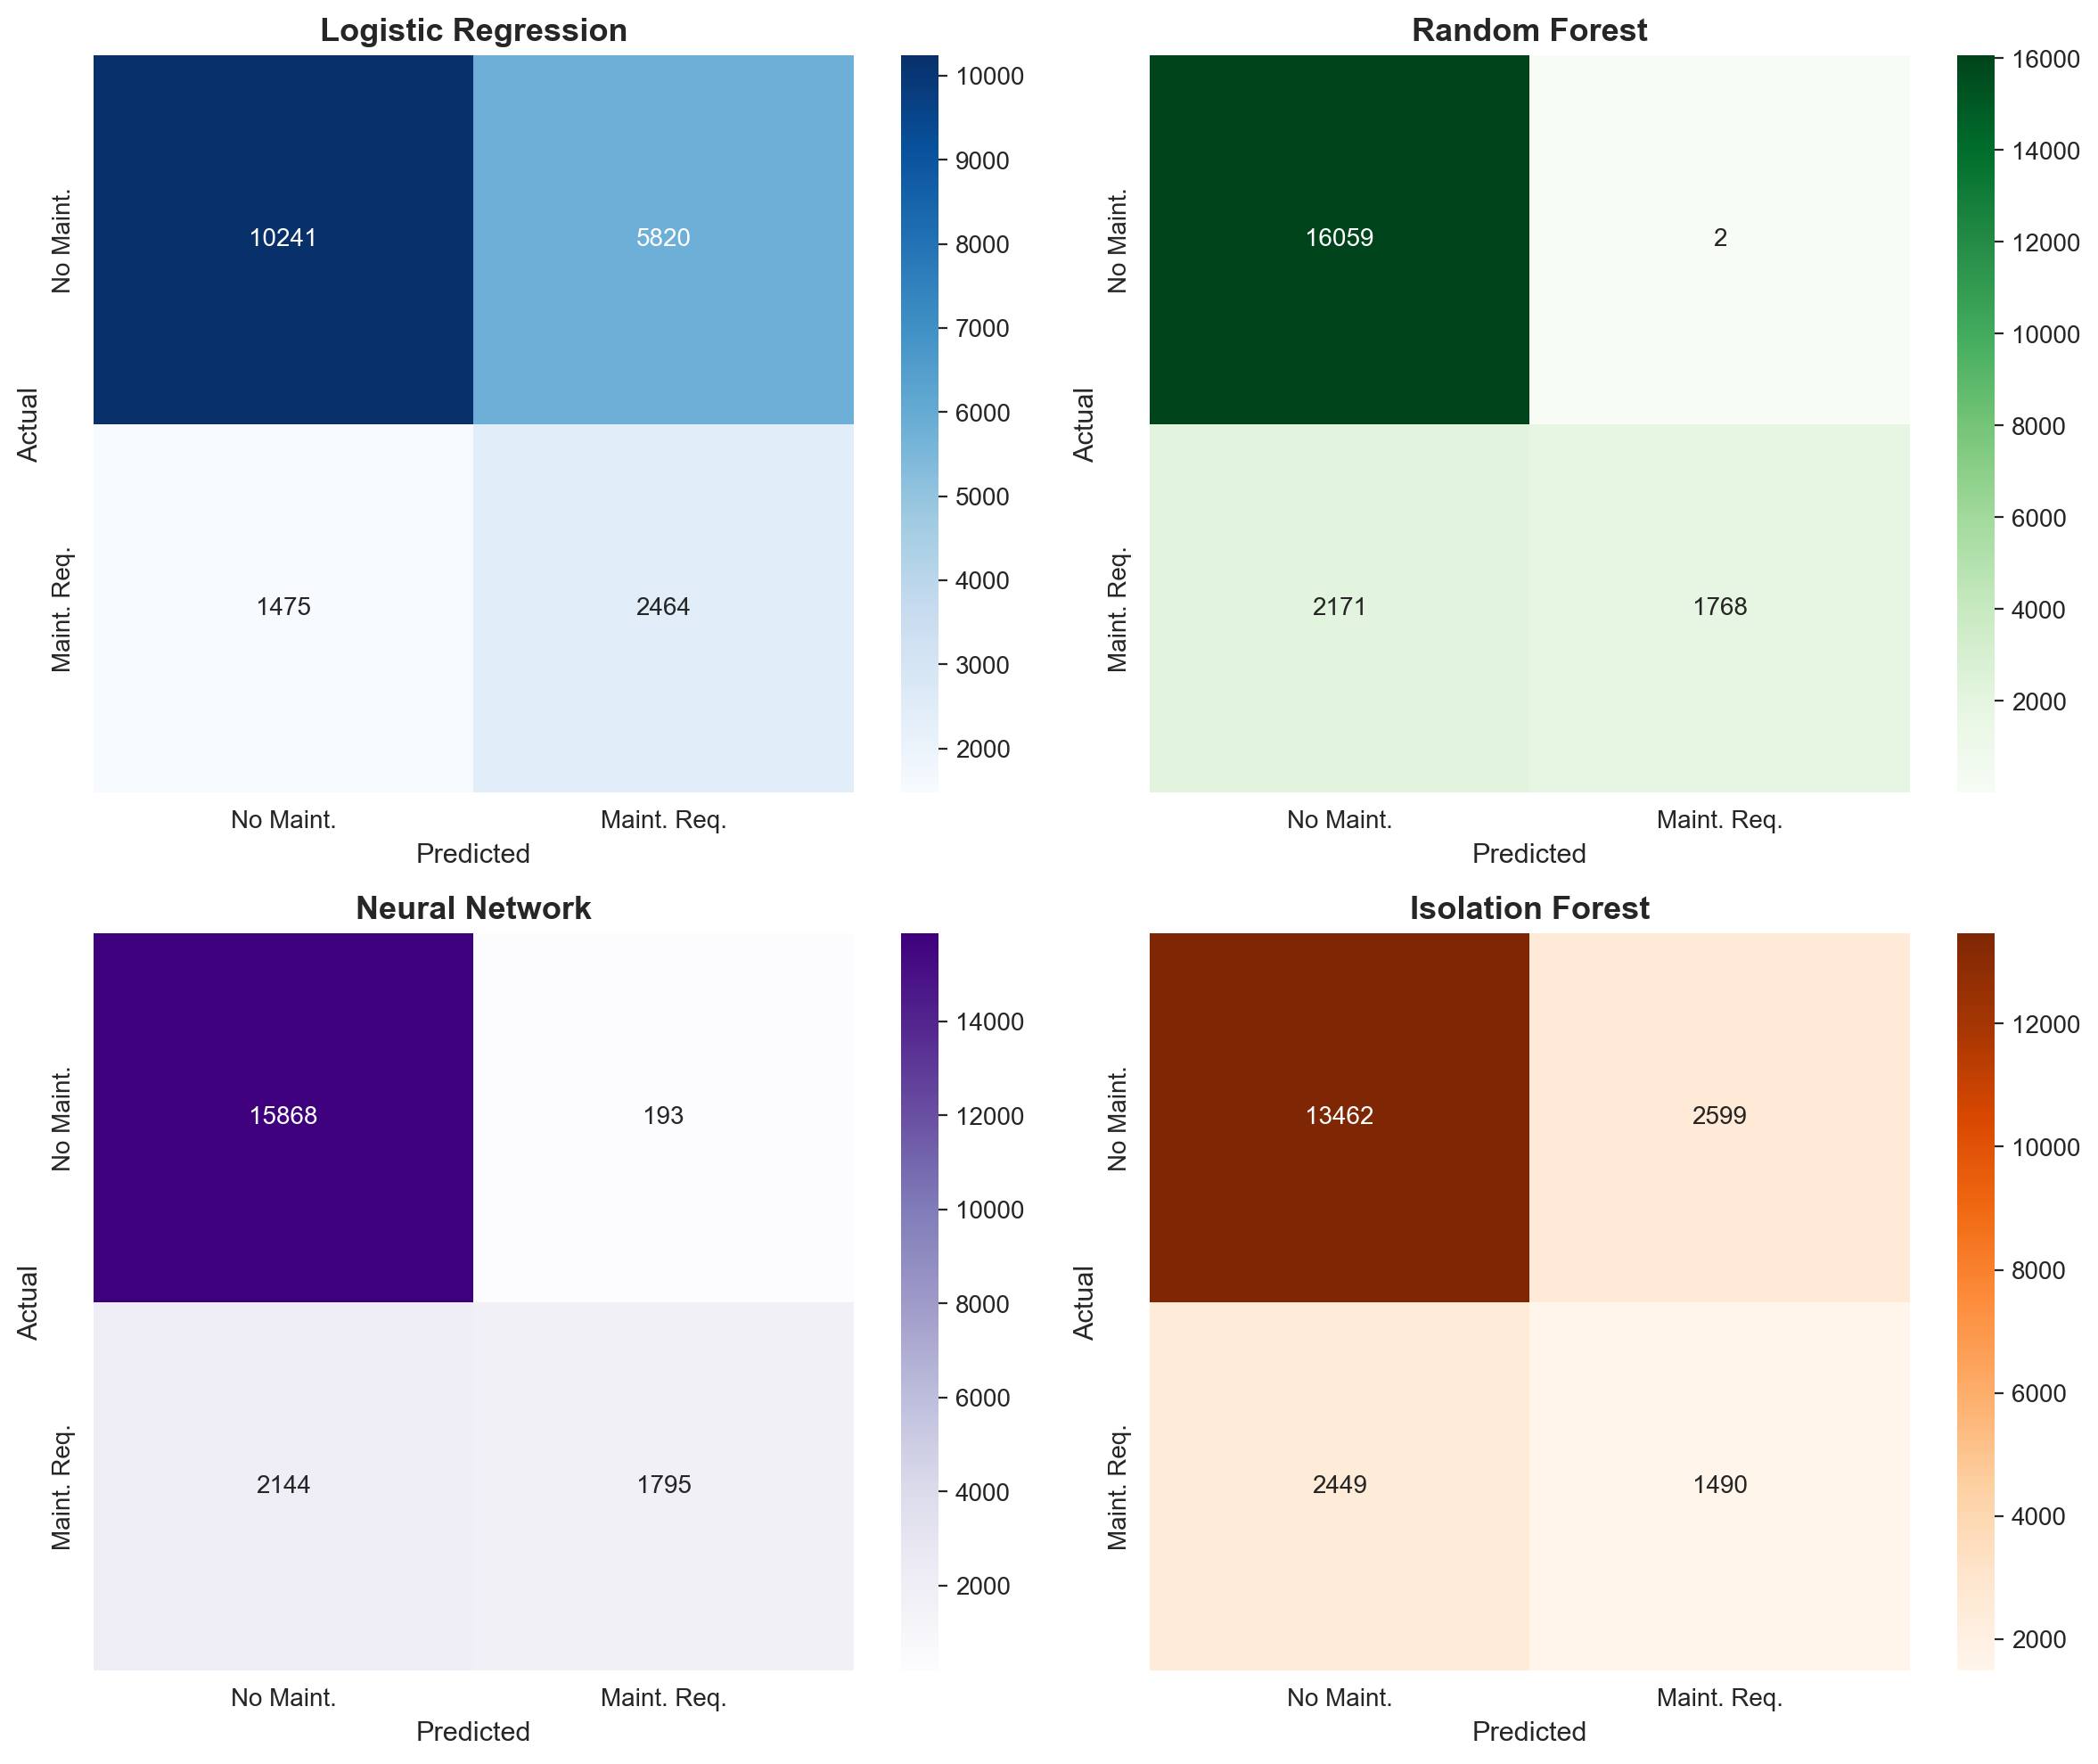
\includegraphics[width=0.55\textwidth]{figures/confusion_matrices.png}
\end{center}
\end{frame}

\begin{frame}{PCA — Variance Analysis}
\begin{columns}[T]
\begin{column}{0.42\textwidth}
{\small
\begin{itemize}\setlength{\itemsep}{2pt}
    \item All \pcaNcomp/5 components needed for 95\% variance
    \item PC1: \pcaVarOne\%, PC2: \pcaVarTwo\% --- nearly uniform
    \item LR+PCA F1 = \pcaFone\ ($\Delta$F1 = $\pcaDeltaF$)
    \item Sensors are nearly orthogonal: no redundancy
\end{itemize}}
\end{column}
\begin{column}{0.54\textwidth}
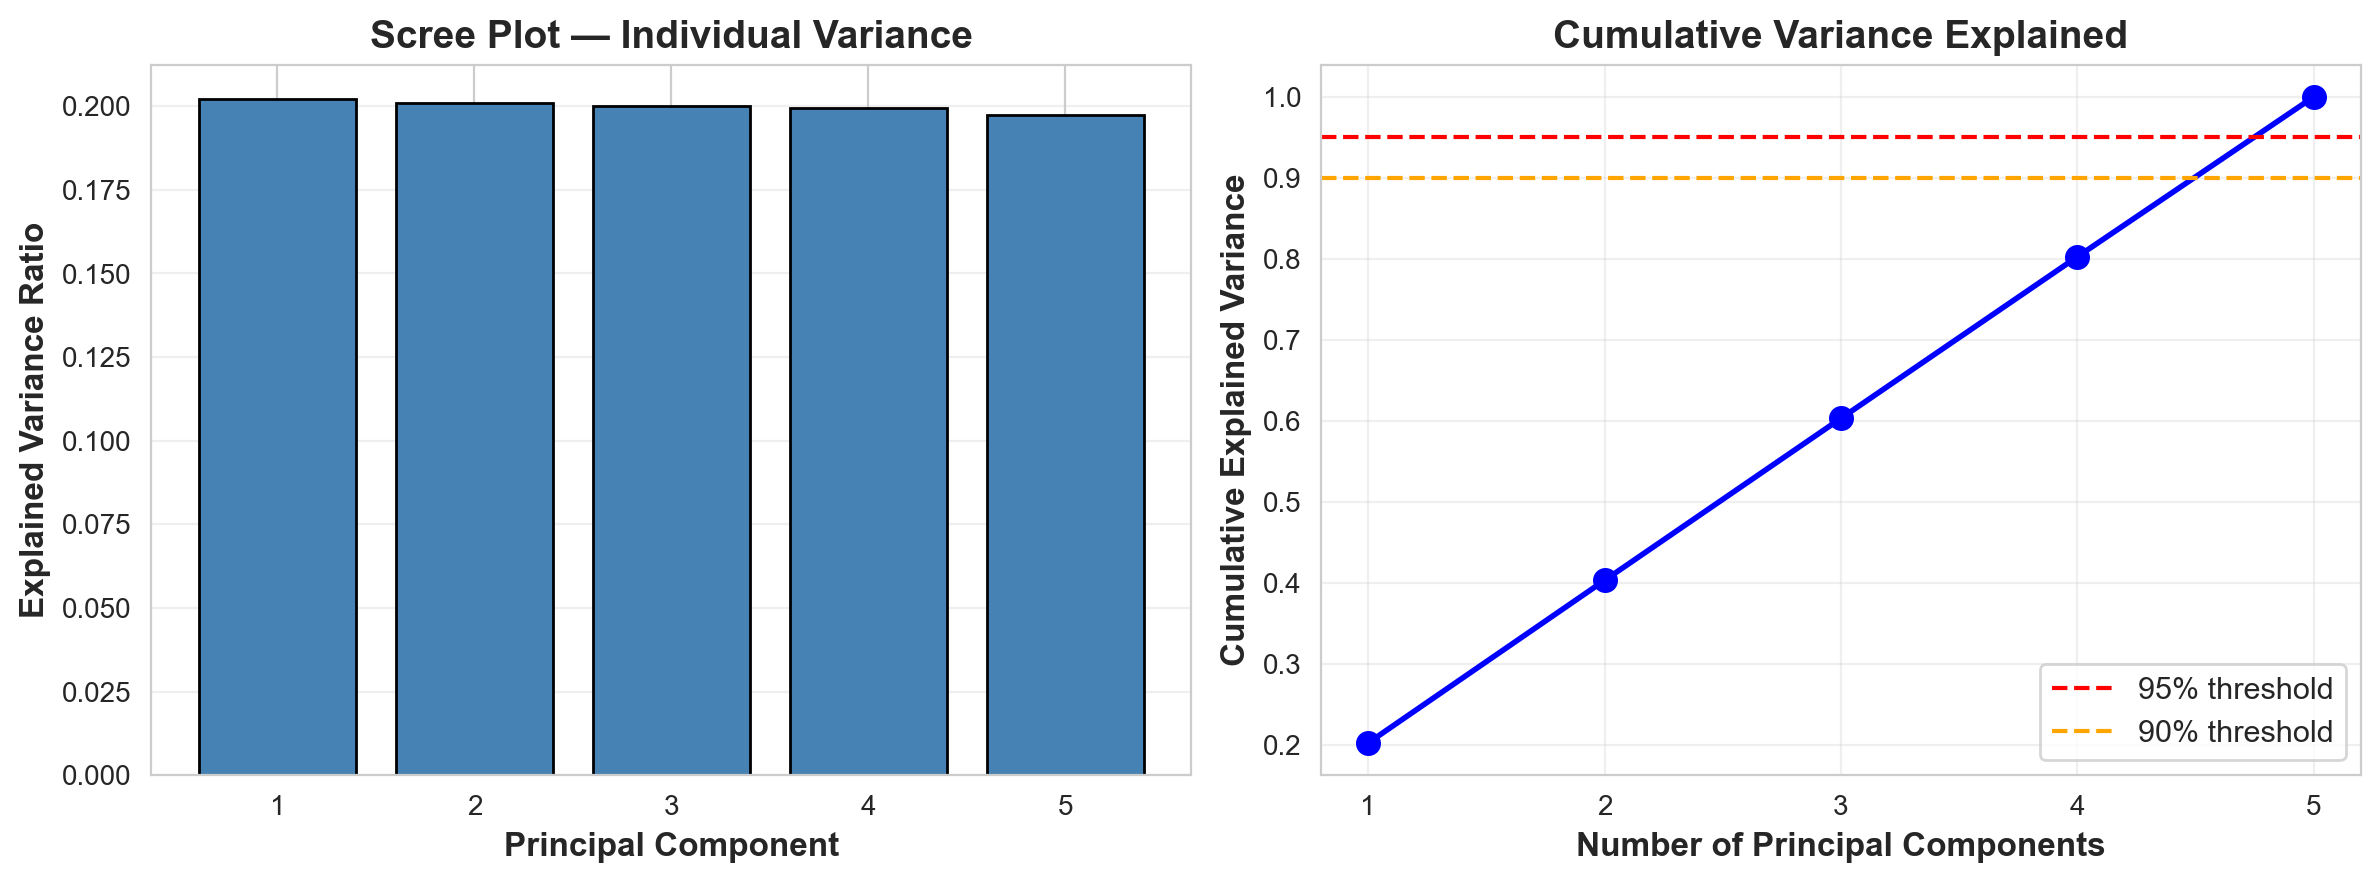
\includegraphics[width=\textwidth]{figures/pca_scree_plot.png}
\end{column}
\end{columns}
\end{frame}

\begin{frame}{Isolation Forest — Unsupervised Anomaly Detection}
\begin{columns}[T]
\begin{column}{0.48\textwidth}
\begin{itemize}
    \item F1 = \isoFone, AUC = \isoAuc\ --- above random (0.5), real signal captured
    \item \isoFP\ false alarms, \isoFN\ missed failures --- balanced error profile
    \item Label value gap: RF F1 \rfFone\ $-$ IF F1 \isoFone\ = 0.25
    \item Viable first-line monitoring when labeled data is unavailable
\end{itemize}
\end{column}
\begin{column}{0.48\textwidth}
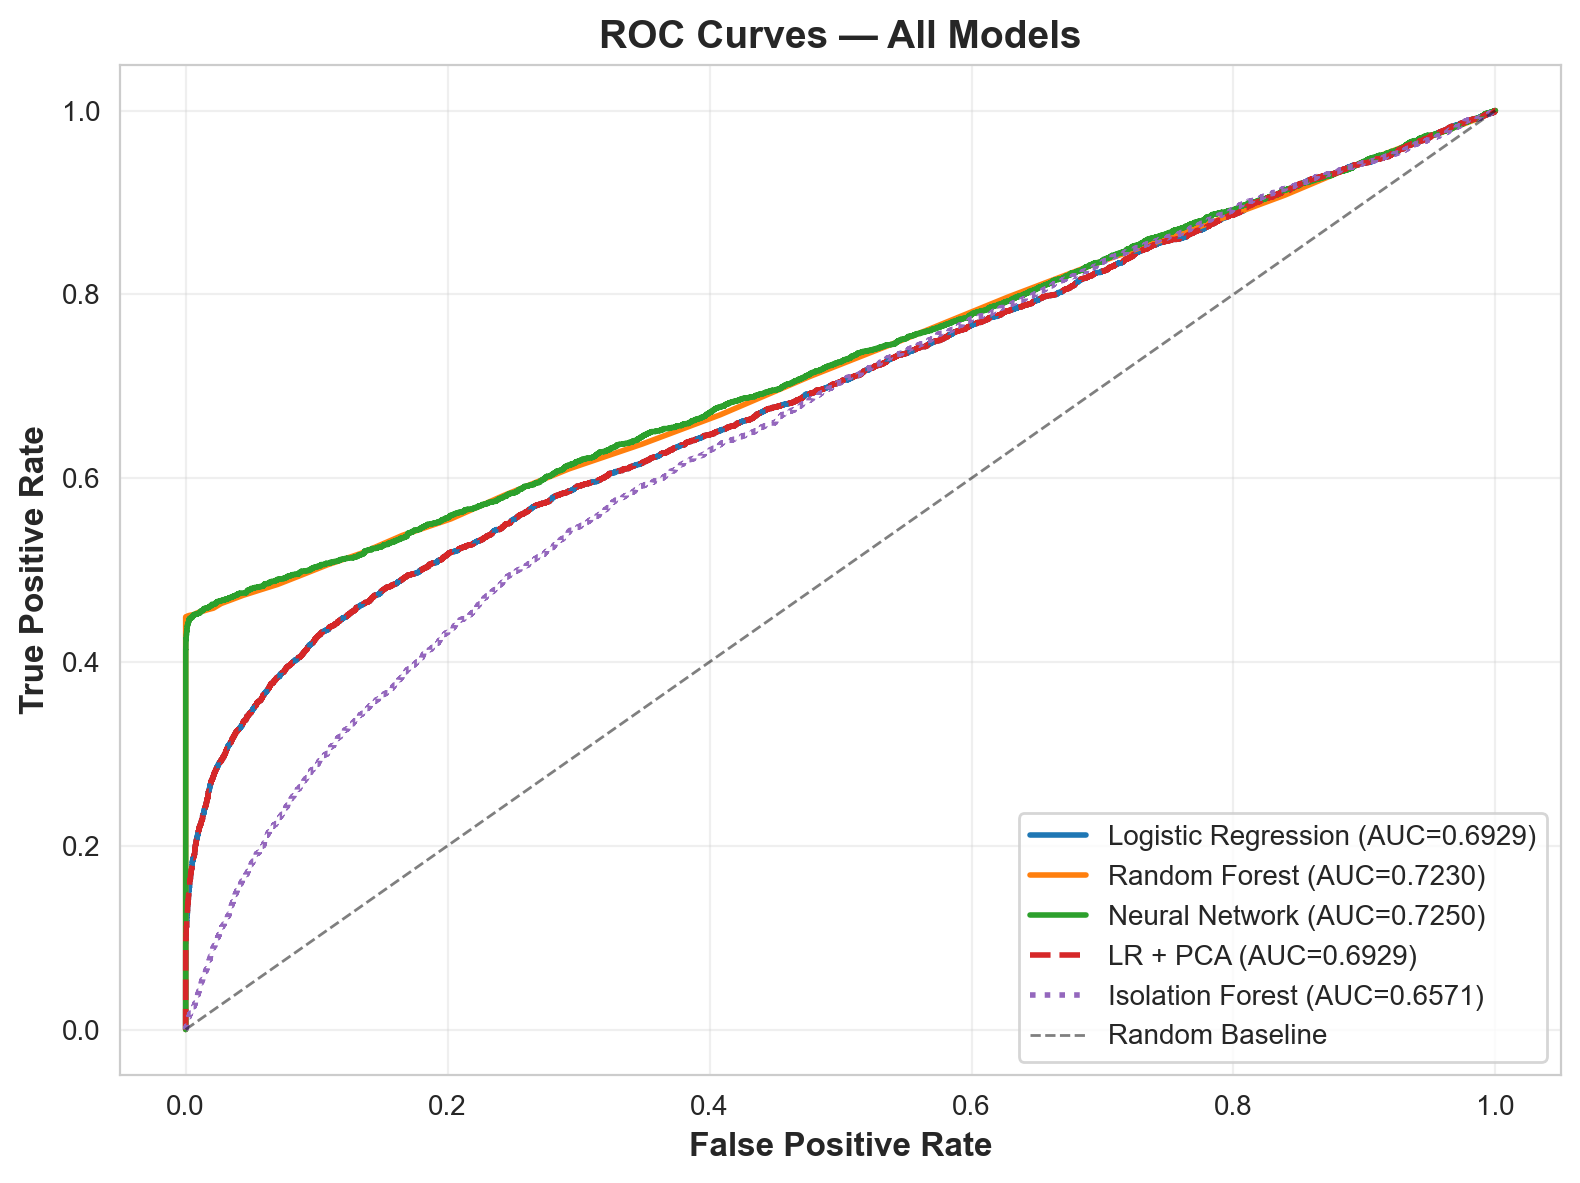
\includegraphics[width=\textwidth]{figures/roc_curves.png}
\end{column}
\end{columns}
\end{frame}

% ============================================================
\section{Discussion}
% ============================================================

\begin{frame}{Strengths \& Limitations}
\begin{columns}[T]
\begin{column}{0.48\textwidth}
\textbf{Strengths:}
\begin{itemize}
    \item Five techniques across model families
    \item Rigorous evaluation (stratified split, CV, multiple metrics, naive baseline)
    \item Data leakage prevention
    \item Hyperparameter tuning \& regularization
    \item Actionable feature importance
\end{itemize}
\end{column}
\begin{column}{0.48\textwidth}
\textbf{Limitations:}
\begin{itemize}
    \item Synthetic dataset --- may not reflect real-world noise
    \item Only 5 raw sensor features; richer engineering possible
    \item No temporal modeling (records treated independently)
    \item Single dataset --- generalizability unvalidated
\end{itemize}
\end{column}
\end{columns}
\end{frame}

% ============================================================
\section{Conclusion \& Future Work}
% ============================================================

\begin{frame}{Conclusion \& Future Work}
\textbf{Key findings:}
\begin{itemize}
    \item RF achieved best F1 (\rfFone) with near-perfect precision (\rfPrec); ANN matched its AUC (\annAuc)
    \item Non-linear models improved F1 by $\sim$50\%  over LR baseline (\lrFone)
    \item Temperature (\rfImpA) and vibration (\rfImpB) account for 58\% of RF's predictive power
    \item PCA: all 5 sensors are non-redundant (each $\approx$20\% variance)
    \item Isolation Forest captures real anomalous structure (AUC = \isoAuc) without labels
    \item Performance ceiling at F1 $\approx$ 0.62 suggests richer features are needed
\end{itemize}

\vspace{0.4cm}
\textbf{Future work:}
\begin{itemize}
    \item LSTM / GRU for temporal degradation patterns
    \item Rolling-window feature engineering from raw sensors
    \item SHAP values for instance-level explainability
    \item Validate on real-world industrial datasets
\end{itemize}
\end{frame}

% ============================================================
\begin{frame}
\centering
\Huge \textbf{Thank You}

\vspace{0.5cm}
\Large Questions?

\vspace{0.5cm}
\normalsize
Group 22 --- MANU 465
\end{frame}

\end{document}
